\chapter{Software Developed}

\section{Python Console}

\section{Verilator Testbench}
\subsection{UUT Top Hardware module}
\label{section:uut}
This top module creates a \textit{verilog} wrapper of the \acrfull{uut} that allows it to interact with the different hardware logic simulators. Even tho this is written harddware logic it is never implemented as real hardware. This module is only used in simulation as software.

The top module file is an adaptation of the previous \textit{verilog} file used on the Icarus simulation. Previously, the verilog top file would interact directly with the console. Similarly to the new hardware top module an \acrshort{uart} module is instantiated and a serial connection with the \textit{IOb-SoC} is simulated. Although in this project the \textit{IOb-UART} in the \acrfull{soc} was swapped for the \textit{UART16550} in the 

\begin{figure}[!ht]
    \centering
    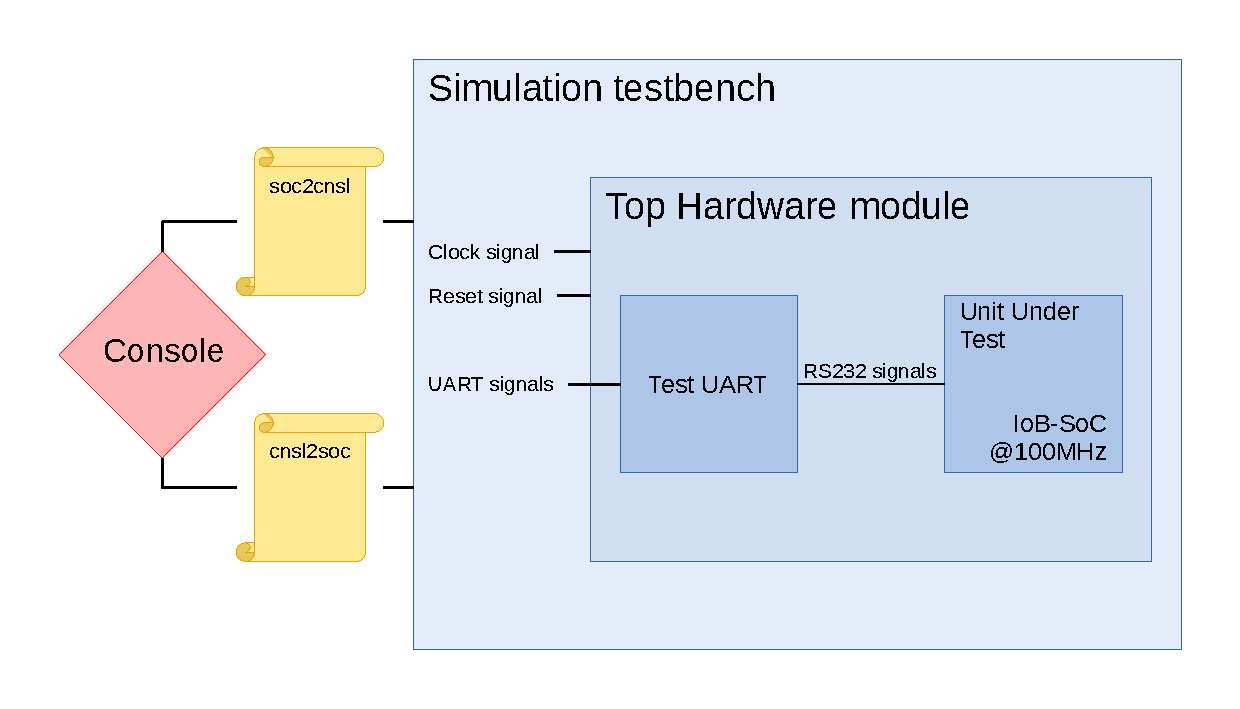
\includegraphics[width=\linewidth]{uut_top_hw.pdf}
    \caption{Simulated hardware interfaces.}
    \label{fig:uut_top_hw}
\end{figure}

\section{Barebones Interrupt Routine}

\section{IOb-SoC Linux Stage 0 Bootloader}

\section{IOb-SoC on OpenSBI}

\section{IOb-SoC Device Tree}

\section{IOb-SoC Linux \textit{'rootfs'}}

\section{Makefiles}